\chapter{Preprocessing}\label{preprocessing}

Le immagini raw nei dataset sono sufficienti ad una \gls{cnn} per ottenere buoni risultati, ma è possibile migliorare i risultati attraverso una pre-eleaborazione delle immagini, in particolare la rimozione di artefatti,  del rumore e migliorare la qualità dell'immagine 
in cui le feacture  possono essere estratte correttamente \cite{permual_contrast}.

\section{Riduzione della risoluzione}\label{riduzione-della-risoluzione}

La rete AlexNet richiede in input una immagine di dimension \(227 \times 227 \times 3\) \cite{alexnet}, dato che le immagini del dataset hanno risoluzione maggiore è stato necessario ridimensionarle alla risoluzione richiesta da AlexNet, questo causa una perdita di qualità dell'immagine, in \cref{fig:resize} si notano due frame: a sinistra con la dimensione originale e a destra ridimensionati, si nota come nonostante la figura ridimensionata è abbastanza accettabile per una elaborazione, nonostante i pixel son ben visibili \cite{gonzalez_dip}.

\begin{figure}[ht]
    \centering
    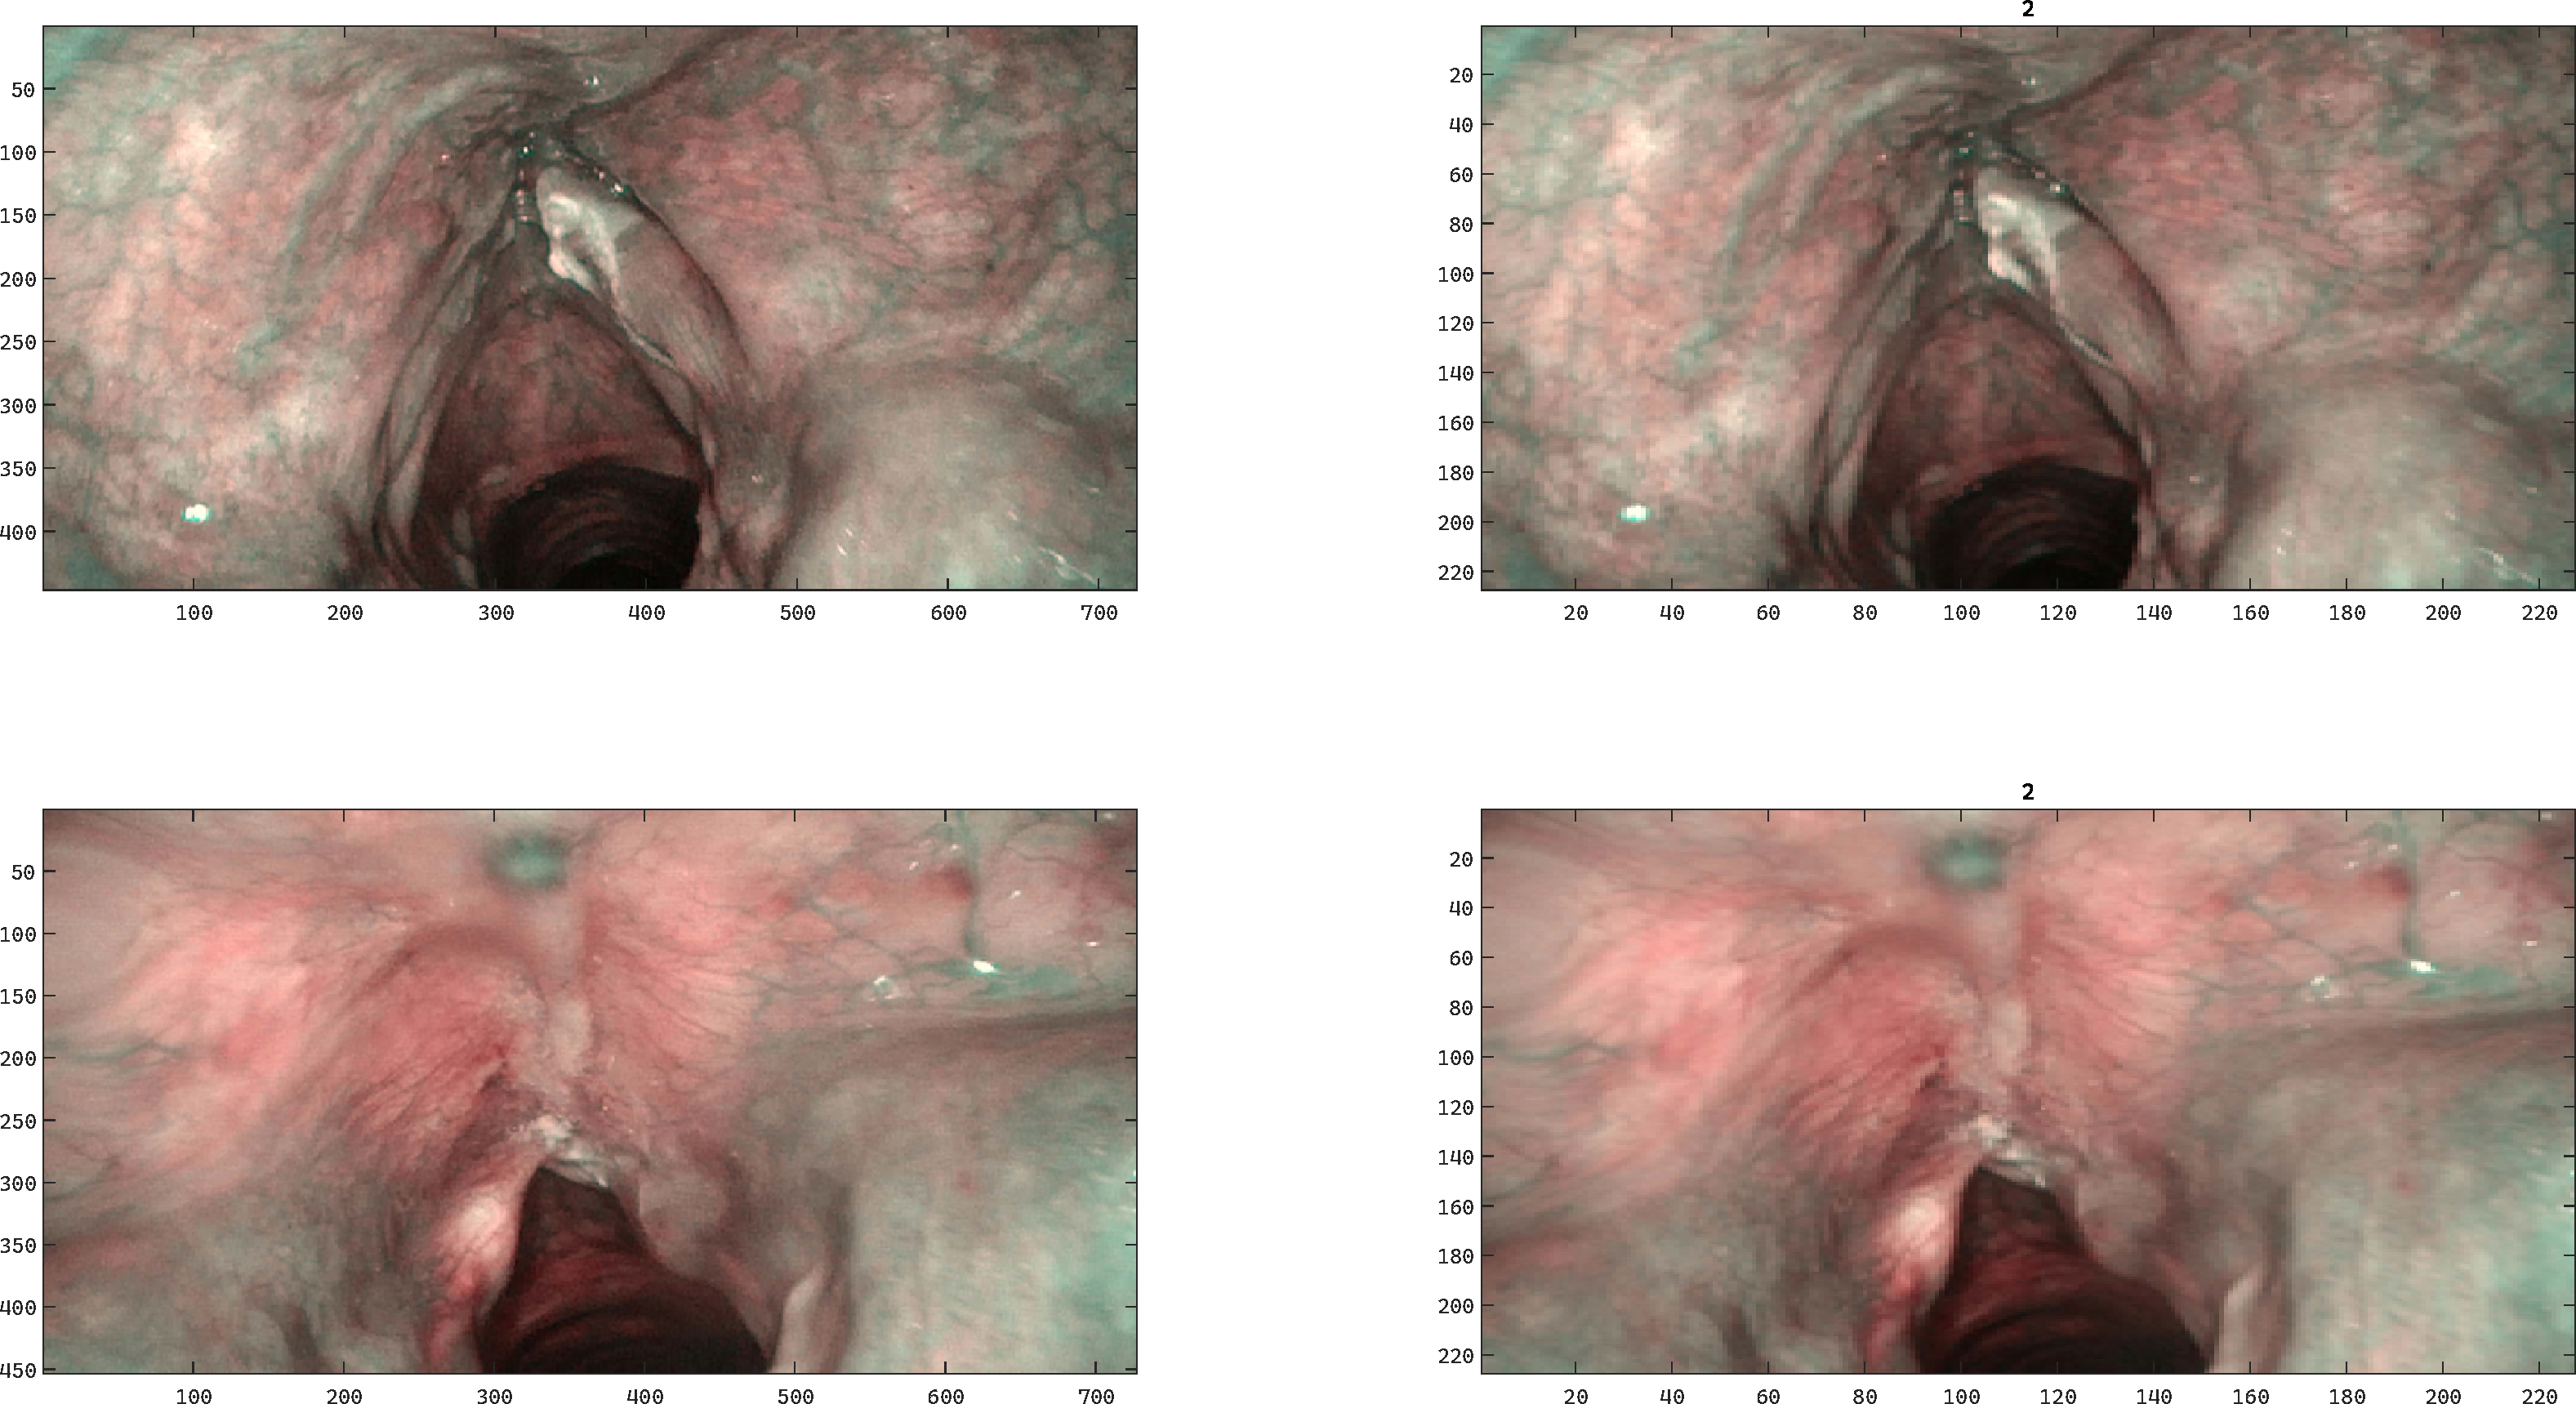
\includegraphics[width=0.7\textwidth]{preprocessing/resize.pdf}
    \caption{Frame del laringoscopio a dimensione intera e ridimensionata}
    \label{fig:resize}
\end{figure}

\section{Contrasto}\label{contrasto}

Il contrasto è la differenza tra la massima e la minima
intensità dei pixel. Si può modificare il contrasto all'immagine per migliorarla secondo determinati valori statici, oppure secondo tecniche più raffinate, per esempio attraverso la deviazione standard e la media. Il contrasto è direttamente correlato all'istogramma dell'immagine. L'istogramma dell'immagine è composto dalle stime della probabilità che l'immagine assuma quel livello, in \cref{fig:histogram-contrast} si nota la correlazione tra l'istogramma ed il contrasto \cite{permual_contrast}  \cite{hummel_histogram} \cite{pandey_contrast} \cite{gonzalez_dip}.

\begin{figure}[ht]
    \centering
    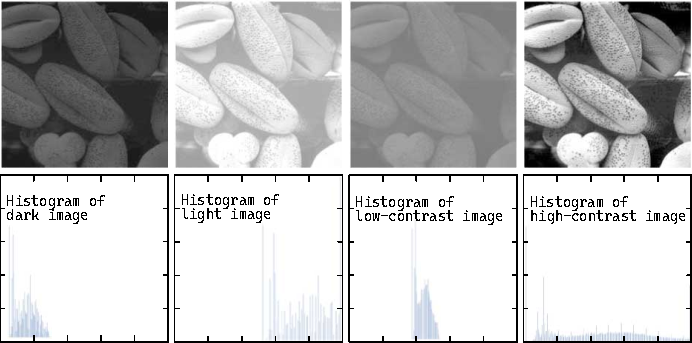
\includegraphics[width=1\textwidth]{preprocessing/histogram-contrast.pdf}
    \caption{Immagine con quattro contrasti diversi e i loro istogrammi corrispondenti}
    \label{fig:histogram-contrast}
\end{figure}

L'algoritmo di ottimizzazione del contrasto è descritto in \cite{gonzalez_dip}, un metodo più raffinato è la stima del MSE e PSNR. Nel processo di miglioramento del contrasto, i pixel con
un valore di colore più basso di un valore specifico vengono visualizzati come
nero, mentre i pixel con un valore di colore più alto vengono
visualizzati come bianco, e i pixel che hanno un valore di colore tra questi due valori vengono visualizzati come una tinta di grigio.
Il risultato di questo processo è una mappatura lineare di un
sottoinsieme di valori che coprono l'intera gamma di grigi da
nero al bianco, creando un'immagine di maggiore contrasto \cite{sunaryo_preprocessing}. 

L'algoritmo per l'ottimizzazione del contrasto è usato per modificare
la gamma dei valori di colore per usare tutti i valori possibili per
migliorare il contrasto. Per preservare l'accurata proporzione del colore
quando viene usato un algoritmo per la  stiratura del contrasto,
viene applicata una stiratura simile per lo stretching di tutti i canali \cite{sunaryo_preprocessing}. 

Nel caso di una immagine a colori, per esempio se i canali rosso e verde sono bilanciati, ma non il canale blu viene allungato l'istogramma del canale blu su entrambi i lati per ottenere
istogramma ben distribuito \cite{sunaryo_preprocessing}.

L'equalizzazione dell'istogramma si può basare, per esempio sul peak signal-to-noise ratio (PSNR), è un indicatore di qualità dell'immagine è calcolato usando l'equazione:

\[ \operatorname{PSNR}=10 \cdot \log _{10}\left(\frac{\operatorname{MAX}_{1}^{2}}{\operatorname{MSE}}\right) \]

Il PSNR è ben definito semplicemente attraverso l'errore quadratico medio (MSE).
Le immagini monocromatiche \(m\times n\) prive di rumore \(\symbfup{I}\) quella originale e \(\symbfup{K}\) quella finale è definita dal MSE:

\[ \operatorname{MSE}=\frac{1}{m n} \sum_{i=1}^{m} \sum_{j=1}^{n}[\symbfup{I}(i, j)-\symbfup{K}(i, j)]^{2} \]

Una volta determinato il PSNR è possibile effettuare una equalizzazione dell'istogramma per aggiustare il contrasto come mostrato in \cref{fig:histogram} \cite{sunaryo_preprocessing} \cite{pandey_contrast} \cite{hummel_histogram}.


\begin{figure}[ht]
    \centering
    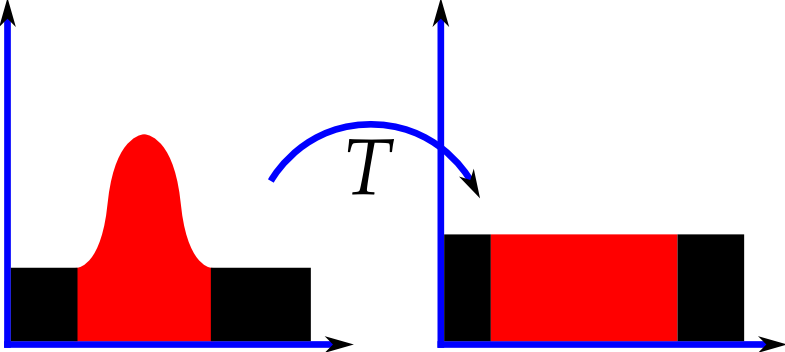
\includegraphics[width=0.5\textwidth]{preprocessing/histogram.png}
    \caption{Metodo dell'equalizzazione dell'istogramma}
    \label{fig:histogram}
\end{figure}



\paragraph{CLAHE}\label{clahe}

Una tecnica più avanzata per migliorare il contrasto nelle immagini è la contrast limited adaptive histogram equalization (CLAHE) che a differenza della classica equalizzazione dell'istogramma divide ogni immagini in tante sotto immagini e per ogni sotto immagine calcola l'istogramma ed effettua il miglioramento del contrasto, come mostrato in \cref{fig:clahe} \cite{hummel_histogram}.


\begin{figure}[ht]
    \centering
    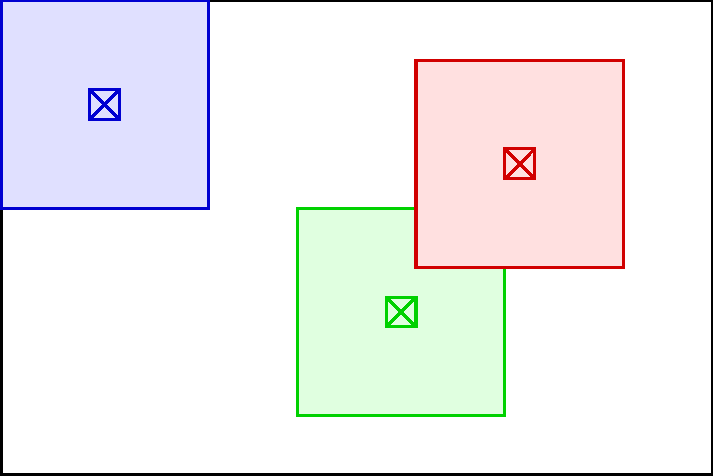
\includegraphics[width=0.5\textwidth]{preprocessing/clahe.pdf}
    \caption{Divisione delle sottoimmagini dell'algoritmo CLAHE che poi vengono equalizzate localmente}
    \label{fig:clahe}
\end{figure}

\section{Gamma}\label{gamma}

La correzione gamma è una correzione non lineare che viene applicata all'immagine per far apparire all'occhio umano le sfumature catturate dalle fotocamere digitali. La correzione gamma si basa sul fato che i nostri occhi non percepiscono la luce come fanno le fotocamere come mostrato in \cref{fig:gamma-correction}, in quanto l'occhio è molto più sensibile ai cambiamenti tra i toni scuri mentre il sensore della fotocamera è molto più lineare e senza la correzione gamma l'immagine risulta più scura del previsto, come mostrato in \cref{fig:gamma} \cite{gamma} \cite{gonzalez_dip}. 

\begin{figure}[ht]
    \centering
    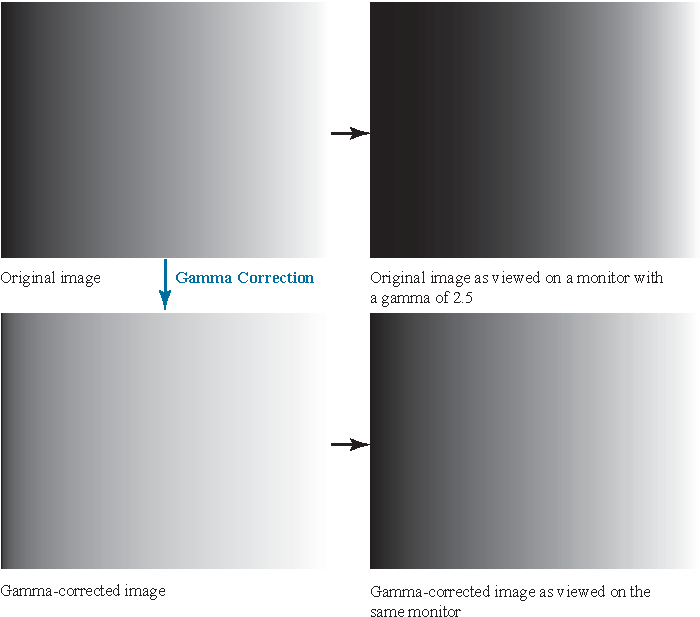
\includegraphics[width=0.7\textwidth]{preprocessing/gamma-correction.pdf}
    \caption{Simulazione di come l'occhio vede l'immagine con e senza correzione gamma}
    \label{fig:gamma-correction}
\end{figure}


\begin{figure}[ht]
    \centering
    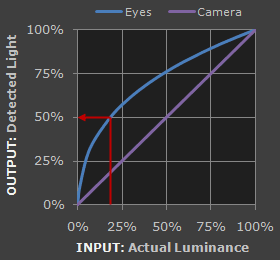
\includegraphics[width=0.5\textwidth]{preprocessing/gamma.png}
    \caption{Luminanza dell'obbiettivo fotografico e dell'occhio umano}
    \label{fig:gamma}
\end{figure}

L'informazione sulla gamma è semplicemente incorporata nei metadata del file e l'immagine viene codificata in maniera lineare, rendendo necessario applicare il filtro gamma in fase di decodifica, è plausibile ipotizzare che pure una CNN funzioni meglio con una immagine preelaborata con un filtro per la gamma \cite{gamma} \cite{gonzalez_dip}.



%\section{Filtro bilaterale}\label{filtro-bilaterale}

%Per la rimozione del rumore  è stato scelto un  filtro bilaterale è stato scelto per la rimozione del rumore perché conserva
%e migliora le caratteristiche che sono utili nelle fasi di addestramento \cite{narbalata_larynge}.